\PassOptionsToPackage{table,xcdraw}{xcolor}
\documentclass{beamer}

\definecolor{mybg}{RGB}{0,102,51}
\definecolor{emcolor}{RGB}{0,0,255}

\mode<presentation>
{
  \usetheme{Frankfurt}      % or try Darmstadt, Madrid, Warsaw, ...
  \usecolortheme{default} % or try albatross, beaver, crane, ...
  \usefonttheme{default}  % or try serif, structurebold, ...
  \setbeamertemplate{navigation symbols}{}
  \setbeamertemplate{caption}[numbered]
  \setbeamertemplate{footline}[frame number]
} 

% beamer stuff
%\useoutertheme[subsection=false]{smoothbars}
%\useinnertheme[shadow=true]{rounded}
%\usecolortheme{seagull}
%\setbeamerfont{block title}{size={}}
%\usefonttheme[onlylarge]{structurebold}
%\setbeamerfont*{frametitle}{size=\normalsize,series=\bfseries}
%\setbeamertemplate{navigation symbols}{}
%\setbeamercolor*{normal text}{fg=white,bg=gray}
%\setbeamercolor*{alerted text}{fg=white}
%\setbeamercolor*{example text}{fg=white}
%\setbeamercolor*{structure}{fg=white}
\AtBeginSection[]
{
  \begin{frame}%<beamer>
    \frametitle{Content}
    \tableofcontents[currentsection,currentsubsection,hideothersubsections]
  \end{frame}
}
% packages
\usepackage{enumerate}
\usepackage[table,xcdraw]{xcolor}
\usepackage{amssymb}
\usepackage{multicol}
\usepackage[normalem]{ulem}
\usepackage{wasysym}
\usepackage{listings}
\lstset{ %
  language=prolog,
%  frame=l,                   			% adds a frame around the code
  basicstyle=\scriptsize\ttfamily,	% use courier
  breaklines=false,
  xleftmargin=0em,
  aboveskip=0.5em,
  belowskip=0.5em,
%  belowcaptionskip=5em,
  numbers=left,
  backgroundcolor=\color{lightgray},
  frame=single,
  framerule=0pt
}
\usepackage{multimedia}
\usepackage{multirow}

% tikz stuff
\usepackage{tikz}
\usetikzlibrary{shadows}
\usetikzlibrary{shapes}
\usetikzlibrary{arrows}
\usetikzlibrary{calc}
\usetikzlibrary{fit}
\usetikzlibrary{backgrounds}
\usetikzlibrary{positioning}
\usetikzlibrary{chains}
\usetikzlibrary{scopes}
\usetikzlibrary{decorations}
\usetikzlibrary{decorations.text}
\usetikzlibrary{decorations.pathmorphing}
\usepackage{animate}

\usepackage{amsmath}
% \usepackage{paralist}

\newcommand{\myemph}[1]{{\bf {\color{emcolor}{#1}}}}

\begin{document}

\title{Towards Knowledge-Intensive Software Engineering}
\author{\myemph{Samuel Cauvin} \and Derek Sleeman \and Wamberto Vasconcelos}
% \author[S.\,Cauvin \& D.\,Sleeman \& W. \,Vasconcelos]
% {%
%   \texorpdfstring{
%       \begin{columns}%[onlytextwidth]
%           \column{.38\linewidth}
%           \centering
%           \myemph{Samuel Cauvin}\\
%           \href{mailto:s.cauvin@abdn.ac.uk}{s.cauvin@abdn.ac.uk}
%           \column{.2\linewidth}
%           \centering
%           Derek Sleeman\\
%           \href{mailto:d.sleeman@abdn.ac.uk}{d.sleeman@abdn.ac.uk}
%           \column{.38\linewidth}
%           \centering
%           Wamberto Vasconcelos\\
%           \href{mailto:w.w.vasconcelos@abdn.ac.uk}{w.w.vasconcelos@abdn.ac.uk}
%       \end{columns}
%   }
%   {Samuel Cauvin \& Derek Sleeman \& Wamberto Vasconcelos}
% }
\institute{
Dept. of Computing Science, University of Aberdeen, Aberdeen, U.K. \href{mailto:s.cauvin@abdn.ac.uk}{s.cauvin@abdn.ac.uk}
}

\date{ICSOFT-EA 2015, Colmar, France\\ \\
\includegraphics[height=1cm]{logo}
\includegraphics[height=1cm,width=2cm]{logo-farr}}

\maketitle

\begin{frame}
  \frametitle{Outline}
  \tableofcontents
\end{frame}

\section{Introduction}
\subsection{}

\begin{frame}
  \frametitle{Introduction}
  Motivation:
  \begin{itemize}
    \item There is a substantial disconnect between software and domain knowledge
    \item Often when developing a system, there already exists an ontology in the same domain
    \item Not making use of this ontology can create inconsistencies
  \end{itemize}
  Proposal:
  \begin{itemize}
    \item Combine code and ontologies with a matching system
    \item Matches shown to the user with reasons, allowing user input
    \item Developed a tool called Facilitator
  \end{itemize}
\end{frame}

\begin{frame}
  \frametitle{Current Landscape}
  Attempts to integrate ontologies and software development:
  \begin{itemize}
	\item A tool, TwoUse combines UML and Ontologies
    \item A second tool, RDFReactor creates Java classes from an Ontology
    \item Another tool finds an ontology for code and then formally relates them together
  \end{itemize}
\end{frame}

\section{Facilitator}
\subsection{}

\begin{frame}
\frametitle{Facilitator Outline}
Facilitator's main functionalities:
\begin{itemize}
\item Finds matches between a Java project and ontologies
\item Displays matches in several ways to the user
\item Creates Java projects from ontologies
\item Creates ontologies from Java projects
\end{itemize}
Facilitator uses an ontology reasoner for some matches.
\end{frame}

\begin{frame}
\frametitle{Screenshot (Parsed Components)}
\centerline{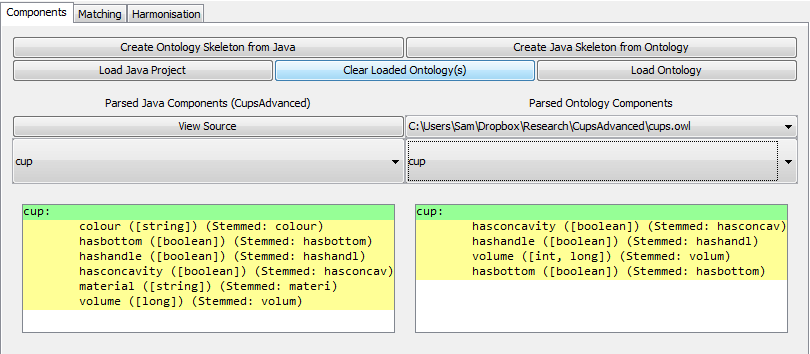
\includegraphics[width=\paperwidth]{ComponentsScreen}}
\end{frame}

\begin{frame}
\frametitle{Screenshot (Match Results)}
\centerline{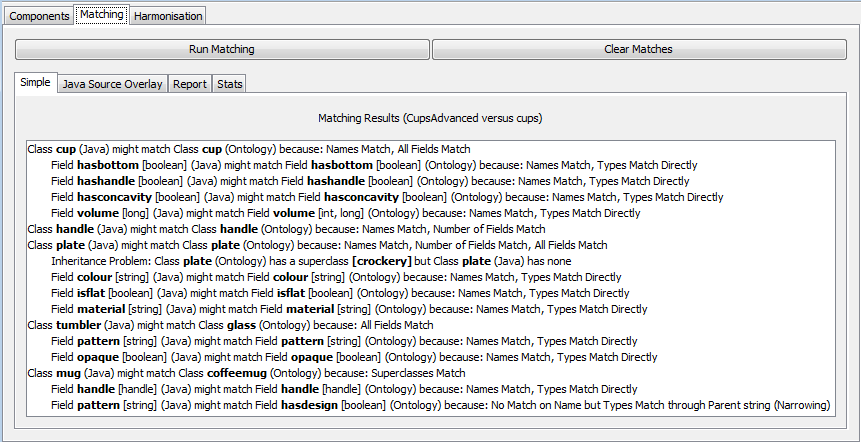
\includegraphics[width=\paperwidth]{MatchingScreen}}
\end{frame}

\begin{frame}
\frametitle{Screenshot (Match Results)}
\centerline{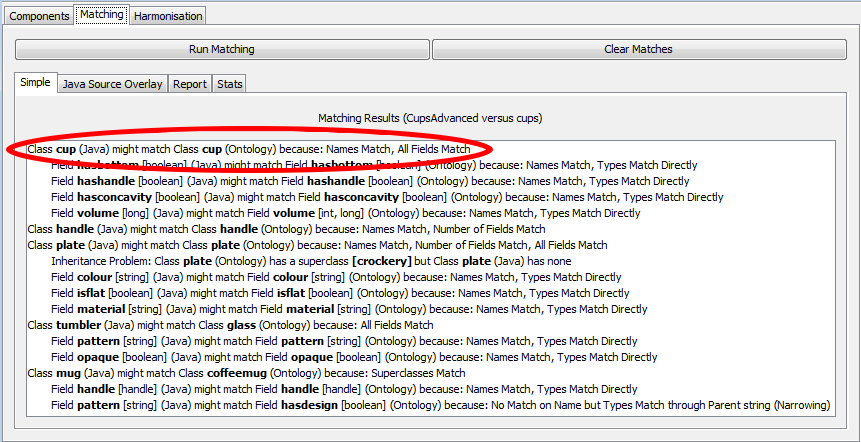
\includegraphics[width=\paperwidth]{MatchingScreen-ClassHighlight}}
\end{frame}

\begin{frame}
\frametitle{Screenshot (Match Results)}
\centerline{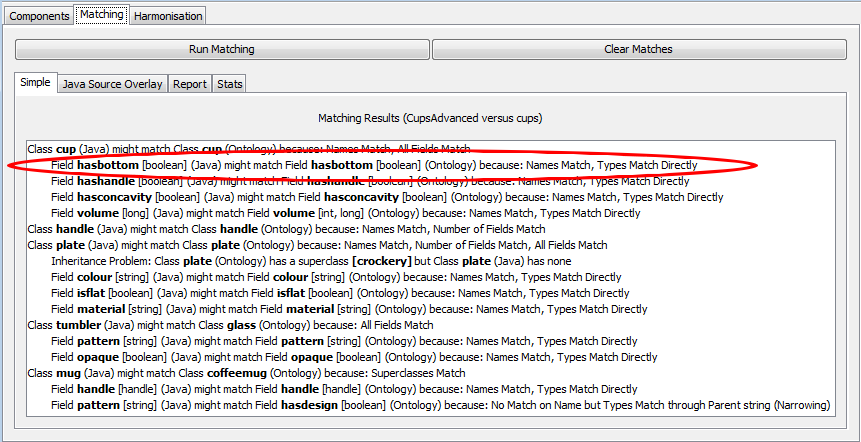
\includegraphics[width=\paperwidth]{MatchingScreen-FieldHighlight}}
\end{frame}

\begin{frame}
\frametitle{Architecture}
\centerline{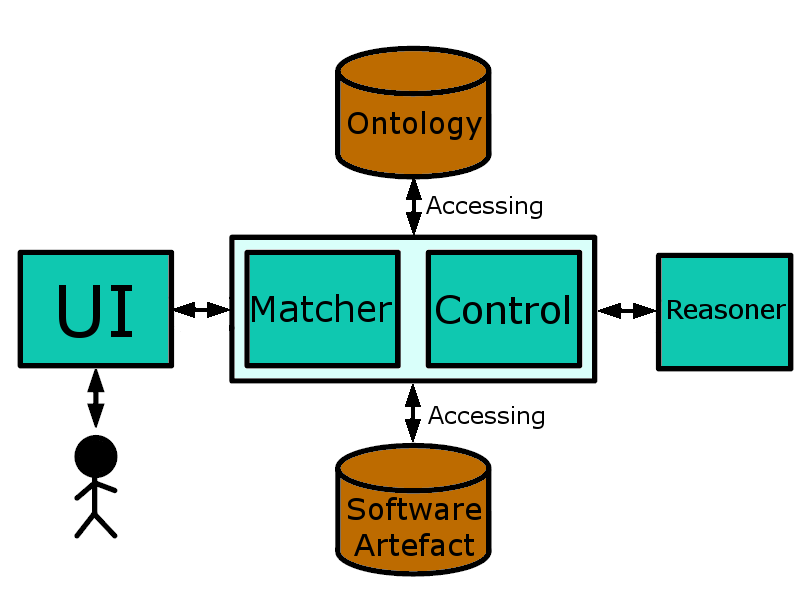
\includegraphics[width=0.9\textwidth]{SoftwareArchitecture}}
\end{frame}

\begin{frame}
\frametitle{Taxonomy of Types}
Facilitator compares data types using a taxonomy of types\newline{}
\newline{}
\centerline{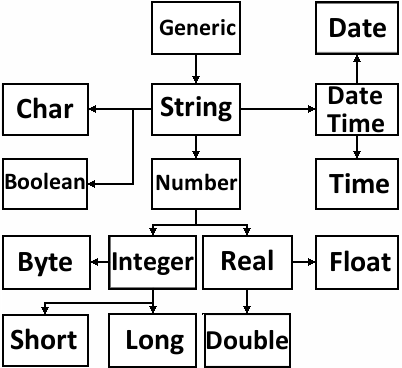
\includegraphics[width=0.6\textwidth]{TaxonomyOfTypes}}
\end{frame}

\section{Matching \& Scenarios}
\subsection{}

\begin{frame}
  \frametitle{Matching Algorithm}
  Matching algorithm has three main stages:
  \begin{enumerate}[1)]
    \item Detecting class matches between class and field names
    \item Detecting class matches using superclass relationships
    \item Detecting field matches, with three sub stages:
    \begin{enumerate}[a)]
      \item Detecting field matches by name and type
      \item Detecting field matches using inferred fields
      \item Detecting field matches by type but not name, exclusively using previously unmatched fields
    \end{enumerate}
  \end{enumerate}
\end{frame}

\begin{frame}
  \frametitle{Illustrative Scenarios: Cars Example}
  %\begin{adjustwidth}{-2em}{-2em}
    \begin{columns}[t]
      \column{.4\paperwidth}
      \begin{table}[h]
      \centering
      \label{my-label}
      \begin{tabular}{|c|l|}
      \hline
      \rowcolor[HTML]{FFCCC9} 
      \multicolumn{2}{|c|}{\cellcolor[HTML]{FFCCC9}Java}                    \\ \hline
      \rowcolor[HTML]{FFCCC9} 
      \cellcolor[HTML]{FFCCC9}                         & String colour      \\ \cline{2-2} 
      \rowcolor[HTML]{FFCCC9} 
      \cellcolor[HTML]{FFCCC9}                         & int wheels         \\ \cline{2-2} 
      \rowcolor[HTML]{FFCCC9} 
      \multirow{-3}{*}{\cellcolor[HTML]{FFCCC9}Car}    & Engine engine      \\ \hline
      \rowcolor[HTML]{FFCCC9} 
      \cellcolor[HTML]{FFCCC9}                         & int horsepower     \\ \cline{2-2} 
      \rowcolor[HTML]{FFCCC9} 
      \multirow{-2}{*}{\cellcolor[HTML]{FFCCC9}Engine} & boolean turbo      \\ \hline \hline
      \rowcolor[HTML]{96FFFB} 
      \multicolumn{2}{|c|}{\cellcolor[HTML]{96FFFB}Ontology}                \\ \hline
      \rowcolor[HTML]{96FFFB} 
      \cellcolor[HTML]{96FFFB}                         & String colour      \\ \cline{2-2} 
      \rowcolor[HTML]{96FFFB} 
      \cellcolor[HTML]{96FFFB}                         & int numberOfWheels \\ \cline{2-2} 
      \rowcolor[HTML]{96FFFB} 
      \cellcolor[HTML]{96FFFB}                         & int horsepower     \\ \cline{2-2} 
      \rowcolor[HTML]{96FFFB} 
      \cellcolor[HTML]{96FFFB}                         & boolean turbo      \\ \cline{2-2} 
      \rowcolor[HTML]{96FFFB} 
      \multirow{-5}{*}{\cellcolor[HTML]{96FFFB}Car}    & int doors          \\ \hline
      \end{tabular}
      \end{table}

      \column{.55\paperwidth}
      \begin{itemize}
      \item Fields with different names but the same type and same class names will be loosely matched if they have not already been matched - Java $wheels$ matched to Ontology $numberOfWheels$, $horsepower$, $doors$.
      \item Java fields with non-primitive types can have the their fields be inferred as fields of the class - fields of Engine inferred as fields of Car.
      \end{itemize}
    \end{columns}
  %\end{adjustwidth}
\end{frame}

\begin{frame}
\frametitle{Illustrative Scenarios: Generic Matching}
      \begin{itemize}
      \item If two classes match, any children of those classes are also likely to match.
      \item If two classes don't match but more than a number of \myemph{fields} match, then the classes are likely to match.
      \item Fields of a superclass can be inferred as fields of its children, and this combined list will be matched with.
      \end{itemize}
\end{frame}

\section{Evaluation}
\subsection{}

\begin{frame}
\frametitle{Performance}
Times for i5 (quad core) 2.5 GHz processor
\begin{itemize}
\item Java Parser: Average $\sim$10,000 lines/sec
	\begin{itemize}
    	\item 19 classes (3,643 lines) in $\sim$0.001 secs
        \item 62 classes (20,007 lines) in 2 secs
        \item 707 classes (216,744) lines in 20 secs
    \end{itemize}
\item Ontology Parser: Average $\sim$800,000 concepts/sec 
	\begin{itemize}
        \item e.g. 2,358 concepts in $\sim$0.001 secs
	\end{itemize}
\item Matching: Average $\sim$20,000 combinations/sec
	\begin{itemize}
    	\item 4 classes (41 lines) matched to 6 concepts in $\sim$0.001 secs
        \item 707 classes (216,744 lines) matched to 743 concepts in 26 secs
	\end{itemize}
\end{itemize}
\end{frame}

\begin{frame}
  \frametitle{User Studies}
  \begin{itemize}
  	\item Subjects: Computing Science final year students
    \item Work in progress, nothing inferred yet as limited meaningful data produced
  \end{itemize}
  Studies:
  \begin{itemize}
    \item Study 1 is designed to test whether Facilitator forms the same matches as users over a given dataset.
    \item Study 2 is designed to test whether Facilitator aids in task completion by having users perform the same task with and without support from Facilitator.
  \end{itemize}
\end{frame}

\section{Contributions \& Future Work}
\subsection{}

\begin{frame}
\frametitle{Contributions}
\begin{itemize}
\item First time that code has been combined with ontologies
\item Facilitator provides a range of integrated functionalities
\item Finds and displays matches between code and ontologies
\item Uses reasoning to form more complex matches
\item Can create code from ontologies
\item Can create ontologies from code
\end{itemize}
\end{frame}

\begin{frame}
\frametitle{Future Work}
Two important functionalities planned for Facilitator:
\begin{itemize}
\item Harmonisation: Carry out changes/corrections to \textit{existing} code based on an ontology, and vice versa. 
\item Ontology/Matching Visualisation: Show ontology in a graphical format overlaid with matching information.
\end{itemize}
\end{frame}

\begin{frame}
\frametitle{Thanks \& Questions}
\centerline{\Huge \myemph{Thanks for your attention!}}

\centerline{\Huge \myemph{Questions?}}
\end{frame}

\end{document}